\chapter{Advanced Topics}
\label{chap:advanced_topics}

In this chapter, we have tried to collect and document a series of advanced topics related to eMoflon and EA.
It is kept rather compact and is meant to be used mainly as a reference, to be consulted on demand when you need it.

\section{Using Enterprise Architect with Subversion}
The following steps are required to setup EA for use with subversion.
This is highly recommended when working in a group and sharing a single EA Project (EAP) file, which is otherwise a huge binary blob.
We assume you wish to use (i) Subversion and (ii) Windows.
For other SCM and operating systems please consult the official documentation from EA.

\subsection{Initial preparation and set-up}

Download and install Slik SVN (mandatory):
\begin{enumerate}
  \item[$\blacktriangleright$] x32: \small{\url{http://www.sliksvn.com/pub/Slik-Subversion-1.6.17-win32.msi}}\\\\
   x64: {\small \url{http://www.sliksvn.com/pub/Slik-Subversion-1.6.17-x64.msi}}
\end{enumerate}

For public/private key authentication, you also need Tortoise SVN:
 
\begin{enumerate}
  \item[$\blacktriangleright$] x32: {\small \begin{minipage}{.95\textwidth}  \url{http://sourceforge.net/projects/tortoisesvn/files/1.6.16/Application/TortoiseSVN-1.6.16.21511-win32-svn-1.6.17.msi/download}
    \end{minipage}}\\\\\\
  x64: {\small\begin{minipage}{.9\textwidth}  \url{http://sourceforge.net/projects/tortoisesvn/files/1.6.16/Application/TortoiseSVN-1.6.16.21511-x64-svn-1.6.17.msi/download}\end{minipage}}
\end{enumerate} 

If you do not want to have your private key password in plain text in an SVN configuration file then also download Pageant:
\begin{enumerate}
  \item[$\blacktriangleright$] {\small \url{http://the.earth.li/~sgtatham/putty/latest/x86/pageant.exe}}  
\end{enumerate}

After installing all the tools we need, we now have to setup the SSH tunnel:
   
\begin{enumerate}
  \item[$\blacktriangleright$] Locate the file \texttt{\%APPDATA\%$\backslash$Subversion$\backslash$config} and open it with your favourite editor. Locate the \texttt{[tunnels]} section.
  \item[$\blacktriangleright$] If you do not want to install Pageant and do not mind entering your password in plain text enter the following command:\\
  \texttt{ssh = "<path to Tortoise SVN>/bin/TortoisePlink.exe" -l \\<username> -pw <password for your private key> -i "<path to your private key>"}
  \item[$\blacktriangleright$] If you wish to use Pageant then the command can be simplified to:\\ \texttt{ssh = "<path to Tortoise SVN>/bin/TortoisePlink.exe" -l \\<username>} as you can add your private key to Pageant.
  \item[$\blacktriangleright$] If you just use direct passwords for authentication then you can leave out the \texttt{-i} option in both cases.
\end{enumerate}

\subsection{How to set-up a version controlled EAP file}
In the following we assume an EAP file has already been placed under version control \emph{according to our tutorial} and that you wish to check-out this file and work with it.
If our instructions do not work, the EAP file might have been placed under version control in a different manner.
If this is the case then please contact whoever checked-in the file and set it up for working with EA and SVN for further instructions.

\begin{enumerate}
  \item[$\blacktriangleright$] Check-out the project with the EAP file from the server using Tortoise-SVN or Eclipse/Subclipse (or any SVN client of your choice). 
  You should now have a \textit{.svn}-folder in the directory where you saved the revision.
  \item[$\blacktriangleright$] Open the EAP file.
  If the EAP file is already under version control \emph{and has been set-up correctly}, a dialogue similar to Fig.~\ref{fig:advanced-topics-eaSVN-incompleteConf} should immediately pop-up. 
  \item[$\blacktriangleright$] Click ``Yes" to open the ``Version Control Settings'' dialogue (Fig.~\ref{fig:advanced-topics-eaSVN-setWorkingCopyPath}).
\begin{figure}[!htbp]
\begin{center}
	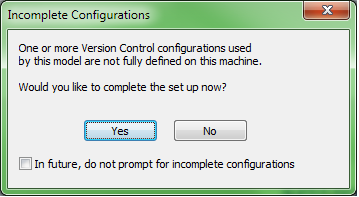
\includegraphics[width=0.5\textwidth]{pics/advancedTopics/eaSVN/DemoLanguages/011}
	\caption{Configure an EAP file which is already under version control}
  	\label{fig:advanced-topics-eaSVN-incompleteConf}
\end{center}
\end{figure}

   \item[$\blacktriangleright$] To work with the EAP file, you now have to \emph{redefine} the SVN variable for the file in your EA workspace. 
   To accomplish this, choose the local path to the folder which contains the EAP file in the ``Working Copy Path'' text-box, and correct the value in ``Subversion Exe Path'' if necessary (to fit your Slik installation location).

\begin{figure}[!htbp]
\begin{center}
	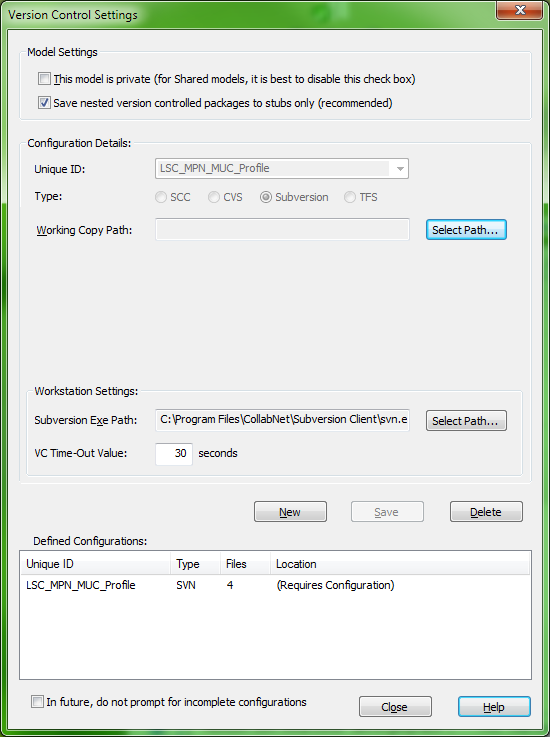
\includegraphics[width=0.5\textwidth]{pics/advancedTopics/eaSVN/DemoLanguages/012}
	\caption{Update settings as required}
  	\label{fig:advanced-topics-eaSVN-setWorkingCopyPath}
\end{center}
\end{figure}

\end{enumerate}
 
\subsection{Working with a version controlled EAP file}
\label{sect:appendixB_update_commit}

\begin{enumerate}
  \item[$\blacktriangleright$] A \texttt{Check Out} retrieves the lock for a certain package and gives you exclusive access, i.e., no one else can change the package. 
  Very important: if subpackages are also under version control, they are not affected by checking out the ``super''-package and remain locked.
  A \texttt{Check Out} also updates the package to the latest version.

\item[$\blacktriangleright$] A \texttt{Check In} commits your work to the server and gives up the lock on the package so others can work on it.
If you do not want to commit your changes, you can just use \texttt{Undo Check Out...} to revert all local changes.

\item[$\blacktriangleright$]  The corresponding \texttt{..Branch} options perform the actions for the current package and all subpackages.
Please note, this has nothing to do with ``branching'' in normal SVN lingo.

\item[$\blacktriangleright$] \texttt{Get Latest/Get All Latest} retrieves the latest version of the selected package / all packages. 
This is basically an update but does not retrieve the lock for any package.

\item[$\blacktriangleright$] Conversely, \texttt{Put Latest} saves all your changes without giving up any locks.

\item[$\blacktriangleright$] \texttt{Compare with controlled version} can be used to review incoming changes. 
Green elements will be added, red will be deleted. 

\item[$\blacktriangleright$] \texttt{File History} gives you a summary of all commits made while you were lying on the beach. 
For a useful file history, always use meaningful commit statements when checking in! 
A date stamp is created automatically.
\end{enumerate}

\subsection{Placing an EAP file under version control}
\label{sect:appendixB_new_EAP_for_vc}

If you already have an EAP file and would like to place it under version control, you first have to check it in as usual on the server using your favourite SVN client. 
Once the project is checked in, the required .svn folder should be in the folder containing the EAP file.
The next step is to register an SVN-variable in EA:
\begin{enumerate}
  \item[$\blacktriangleright$] Open the EAP file, right click on a root folder and select ``Package Control'' and then ``Version Control Settings...'' (Fig.~\ref{fig:advanced-topics-eaSVN-rightclick}).
\begin{figure}[!htbp]
\begin{center}
 	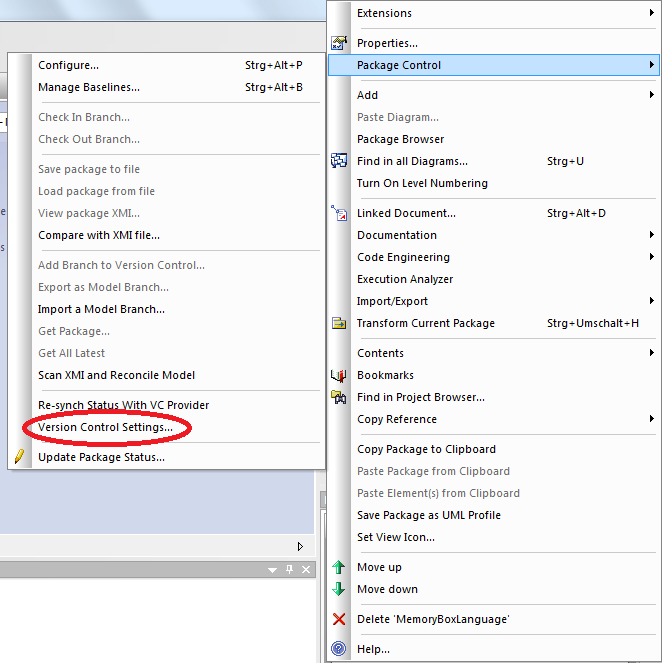
\includegraphics[width=0.7\textwidth]{pics/advancedTopics/eaSVN/rightclick}
	\caption{Select version control settings}
  	\label{fig:advanced-topics-eaSVN-rightclick}
\end{center} 
\end{figure}
  \item[$\blacktriangleright$] In the dialogue, choose a unique ID of your choice (we suggest you use the name of the EAP file) for the settings and activate the ``Subversion'' radio button below.
  \item[$\blacktriangleright$] Choose the local path to the folder which contains the EAP file in the ``Working Copy Path'' text-box.
  \item[$\blacktriangleright$] The field ``Working Station'' must point to where you installed Sliksvn, i.e., \texttt{<path to SlikSVN>$\backslash$bin$\backslash$svn.exe")}.  
  Press ``Save'' and close the dialogue (Fig.~\ref{fig:advanced-topics-eaSVN-variable}).
  If the dialogue closes without an error message, then you can be sure to have configured everything correctly.
%\usepackage{graphics} is needed for \includegraphics
\begin{figure}[!htbp]
\begin{center}
	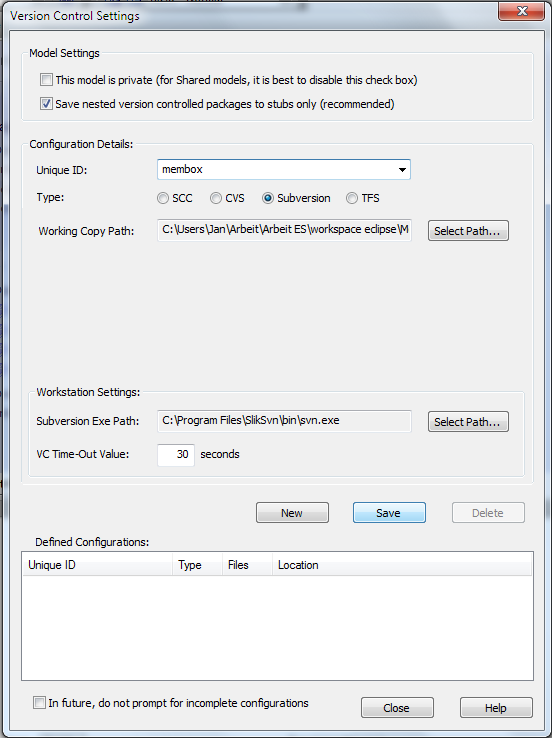
\includegraphics[width=0.6\textwidth]{pics/advancedTopics/eaSVN/versioncontrol}
	\caption{Register an SVN variable in EA}
  	\label{fig:advanced-topics-eaSVN-variable}
\end{center}
\end{figure}
\item[$\blacktriangleright$] In the EAP file, choose ``Package Control$\backslash$Configure...'' for \emph{each package} you wish to place under version control. 

\item[$\blacktriangleright$] In the ensuing dialogue, activate ``Control Package'' and select your previously defined SVN variable from the drop-down menu. 
Enter the path where the XML file for the project should be placed.
Although this is not enforced in any way, we recommend you create a folder structure that mirrors the package structure in EA (Fig.~\ref{fig:advanced-topics-eaSVN-addPackage}).
This process has to be repeated \emph{for all sub-packages} as soon as their super-package has been placed under version control.
\begin{figure}[!htbp]
\begin{center} 
	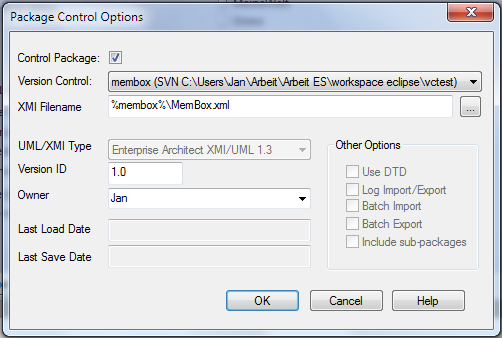
\includegraphics[width=0.6\textwidth]{pics/advancedTopics/eaSVN/cont}
	\caption{Placing a package under version control}
  	\label{fig:advanced-topics-eaSVN-addPackage}
\end{center}
\end{figure} 

\item[$\blacktriangleright$] As a final step, check-in the current state of the EAP file directly with your SVN client. 
As from this point, the EAP file should not be checked-in anymore, and all versioning actions should be performed via EA (and not directly with your SVN client).
\end{enumerate}

\section{Conditional branching and operation results}
During the development of a model transformation with the SDM-language, one eventually encounters a situation where one needs to chose among two patterns based on the return value of an arbitrary operation invocation.
Think, for example, of the situation where you have a class \texttt{A} comprising an operation \mbox{\texttt{doSomeCheck(p$_1$,\ldots,p$_n$ :EClass) :EBoolean}}
which might either encapsulate hand-written java code or be derived from another SDM specification. One possibility to achieve the required branching would lie in assigning the returned value to some dummy attribute (via \emph{attribute assignment}) of
the object of type \texttt{A} (the one, on which we invoked the method). In an immediately following pattern one could then check, whether the \texttt{A} instance carries the expected result in its dummy variable (via \emph{attribute value expression} and comparison to a boolean literal) and branch as done before by using \emph{success} and \emph{failure} edges.

This detour based on a dummy variable has the drawbacks of polluting the metamodel with helper variables induced by technical shortcomings and of concealing the connection between the conditional branch and its condition. It is why we introduced the option to SDM to branch the control flow based on the result of an operation invocation within a \emph{StatementNode} - but only if the return type of the method is specified to be of type EBoolean (other return types could be converted to an EBolean representation by another helper operation though).

Fig.~\ref{fig:cond_branch_on_op} shows a simplistic metamodel and an usage example for the presented SDM language feature. Fig.~\ref{fig:cond_branch_on_op_code} depicts the relevant code sections after code generation. 

\begin{figure}[htp]
\begin{center}
  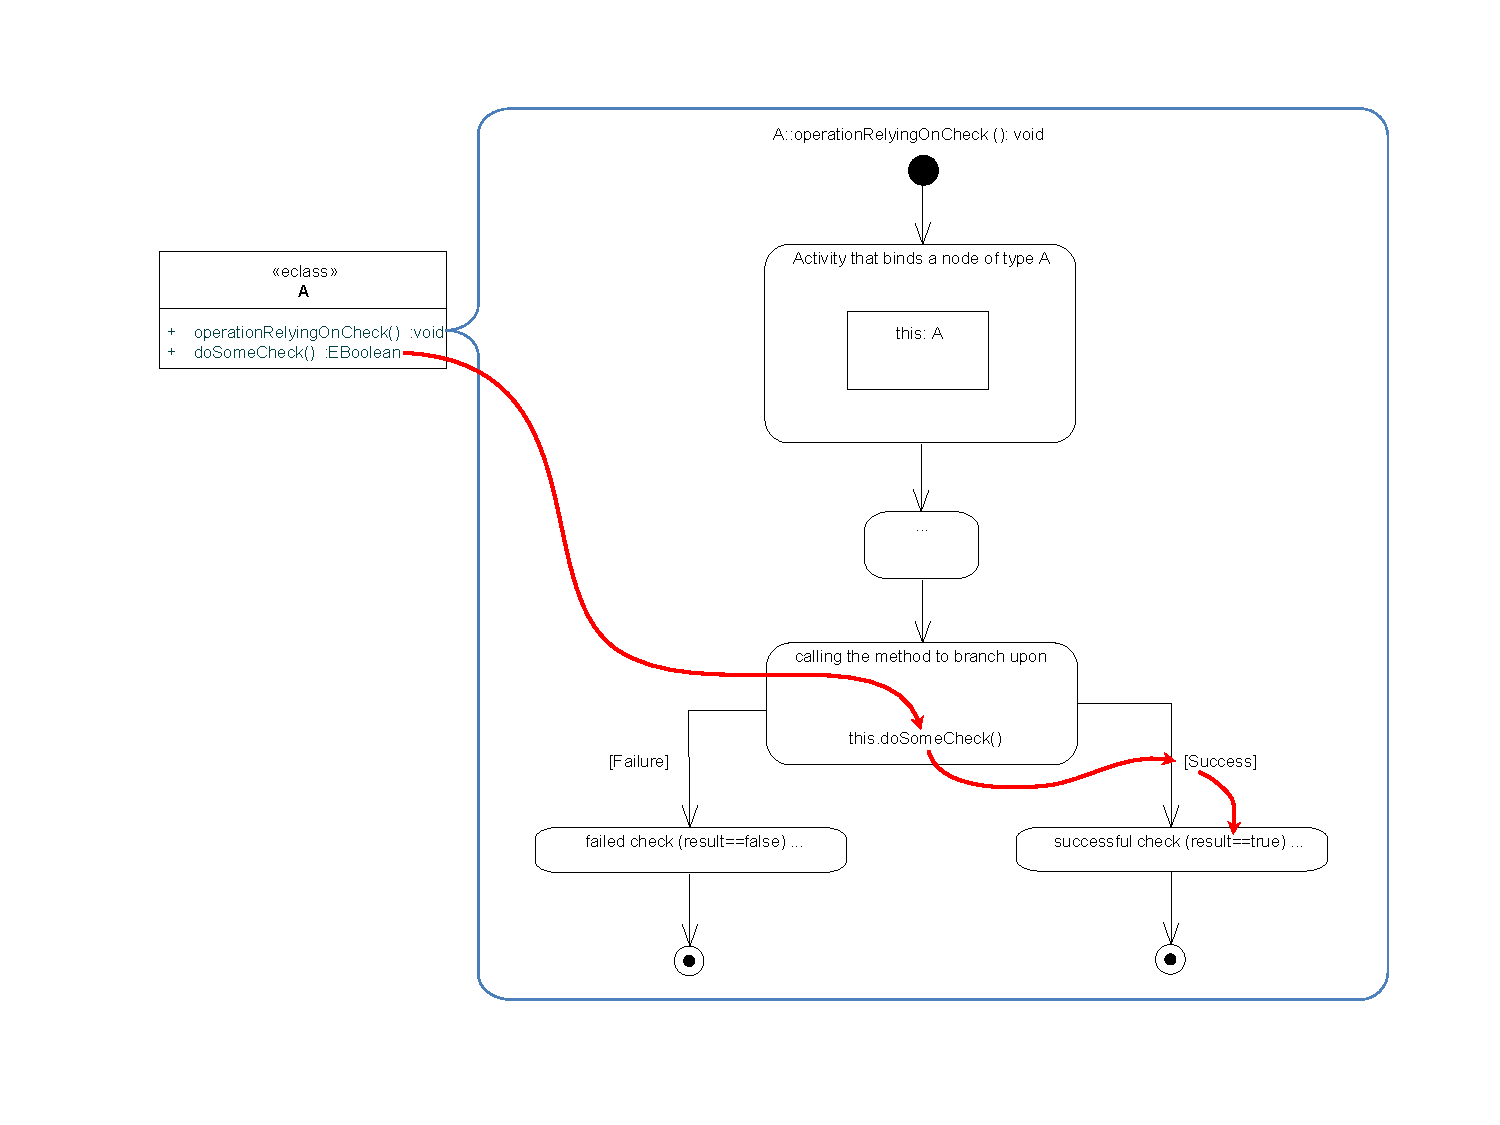
\includegraphics[width=1\textwidth]{pics/advancedTopics/branching/SDM_with_branch}
  \caption{Conditional branching based on result of an operation}
  \label{fig:cond_branch_on_op}
\end{center}
\end{figure}

\begin{figure}[htp]
\begin{center}
  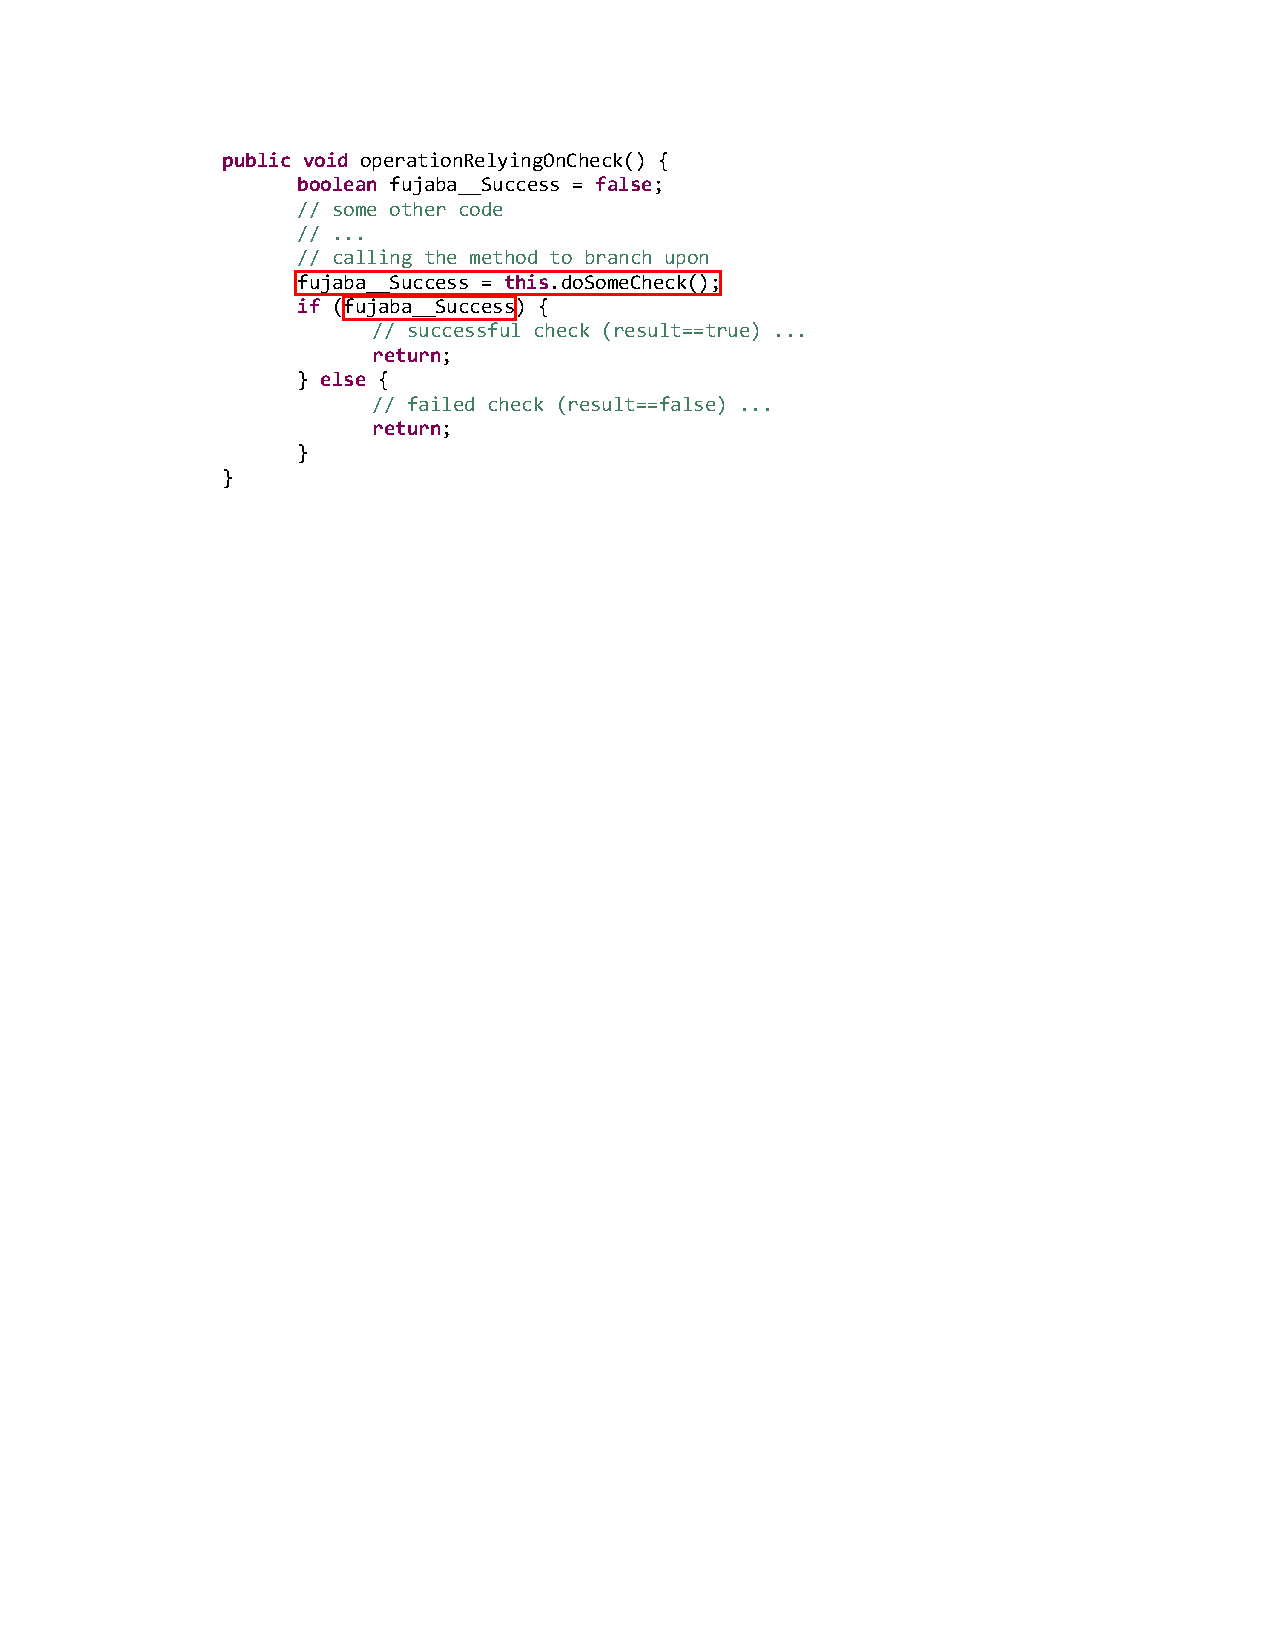
\includegraphics[width=0.7\textwidth]{pics/advancedTopics/branching/generated_code}
  \caption{Generated code}
  \label{fig:cond_branch_on_op_code}
\end{center}
\end{figure}

The key tasks of workflow to get there are as follows:

\begin{enumerate}
\item[$\blacktriangleright$] Locate the position of the required branch and add a new statement node (cf.~fig.~\ref{fig:cond_statement_node}).
\item[$\blacktriangleright$] Specify the right method (corresponding to an operation in the metamodel with \texttt{EBoolean} return type) to be invoked (cf.~fig.~\ref{fig:cond_method_call}). 
\item[$\blacktriangleright$] Add departing \texttt{success} \emph{and} \texttt{failure} edges to the statement node.
\item[$\blacktriangleright$] The \texttt{success} edge is taken if the method returns \texttt{true}, else the \texttt{failure} edge is taken.
\end{enumerate}

\begin{figure}[htp]
\begin{center}
  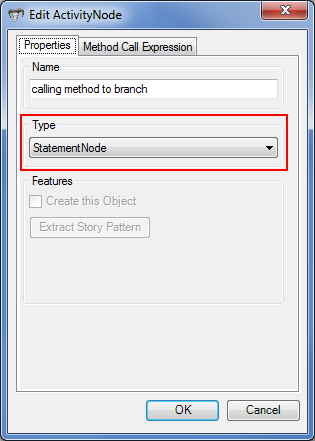
\includegraphics[width=0.5\textwidth]{pics/advancedTopics/branching/01_switch_to_statement_node}
  \caption{Switch from activity node to statement node}
  \label{fig:cond_statement_node}
\end{center}
\end{figure}

\begin{figure}[htp]
\begin{center}
  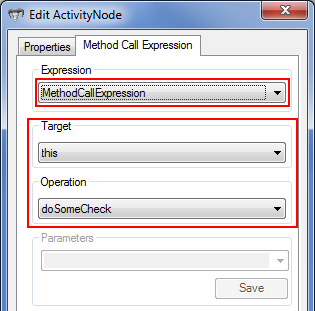
\includegraphics[width=0.5\textwidth]{pics/advancedTopics/branching/02_specify_method_call_expression}
  \caption{Specify the method call expression}
  \label{fig:cond_method_call}
\end{center}
\end{figure}